\documentclass[10pt,a4paper]{scrartcl}
\pagestyle{empty}
\usepackage{a4} % alternativ \usepackage{a4wide}
\usepackage[ngerman]{babel} % Neudeutsche Silbentrennung (mehrsprachiges Dokument)
\usepackage{parskip} % Skip indentation of first row
\usepackage{graphicx} % Graphics support
\usepackage{longtable} % Tables across several pages
\usepackage{booktabs}
\usepackage{hyperref} % Hyperlinks
\usepackage[automark]{scrpage2} %kopf/fusszeile
\usepackage[utf8x]{inputenc} % Unicode-Encoding
 
\linespread{1.3}

\author{Danilo Bargen, Christian Fässler, Jonas Furrer} 
\title{Domainanalyse\\Projekt BierIdee}

\pagestyle{scrheadings}
\ihead{SE2 Projekte} %linke Kopfzeile
\ohead{BierIdee} %rechte Kopfzeile

\begin{document}

\begin{titlepage}
	\maketitle
	\vspace{120mm}
	\thispagestyle{empty} % Don't start page numbers on this page
\end{titlepage}

\tableofcontents
\newpage

\section{Änderungshistorie}
\begin{tabular}{p{0.1\textwidth}p{0.15\textwidth}p{0.55\textwidth}p{0.1\textwidth}}
\toprule
\textbf{Version} & \textbf{Datum} & \textbf{Änderung} & \textbf{Person} \\  
\midrule
v1 & 26.03.2012 & Dokument erstellt & jfurrer \\  
\hline 
v1.1 & 31.03.2012 & Korrekturen nach Review & jfurrer \\
\bottomrule
\end{tabular} 
\newpage

\section{Einführung}
\subsection{Zweck}
Dieses Dokument zeigt den Aufbau der Domain des Projekts "BierIdee".

\subsection{Gültigkeitsbereich}
Die Gültigkeit dieses Dokumentes erstreckt sich über die Dauer der Planung und Umsetzung des Projektes und beschränkt sich auf die Dauer des Modules SE2 Projekte FS2012.

\subsection{Referenzen}
\begin{itemize}
	\item Glossary.pdf
	\item Usecases.brief.pdf
	\item Usecases.fully.dressed.pdf
\end{itemize}

\subsection{Übersicht}
Im ersten Teil des Dokumentes wird die Domain analysiert und aufgezeichnet, darauf folgend werden die Systemsequenzdiagramme von zwei zentralen Usecases betrachtet. Im letzten Teil werden die Contracts der Systemoperationen der beandelten Systemsequenzdiagrammen besprochen.


\section{Domainalayse}
\subsection{Domainmodel}
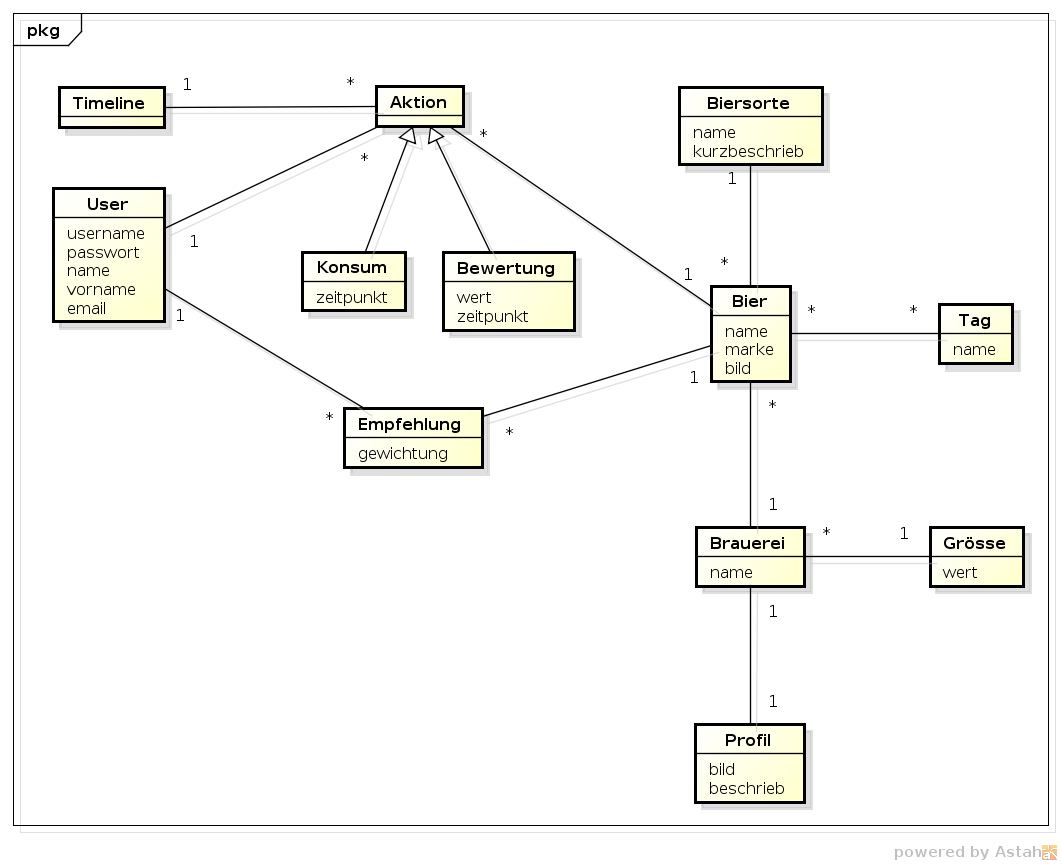
\includegraphics[width=\textwidth]{domain_model_bieridee.png} 

\subsection{Begrifferläuterung}
In der folgenden Liste werden Domainklassen und -attribute genauerbeschrieben. Es finden sich nicht alle Klassen und Attribute in der Liste, sonder nur solche die nicht komplett selbsterklärend sind.
\begin{description}
	\item[Bier] Dies bezeichnet ein Bier, welches sich über das Bierrezept definiert. Konkret beispielsweise eine Flasche Appenzeller Quöllfrisch oder eine Büchse Feldschlösschen Premium. Die Verpackung spielt dabei keine Rolle.
	\begin{description}
	\item[marke] Bei der Marke handelt es sich um einen String der die Biermarke beschreibt. Oft wird die Marke und die Brauerei identisch sein, das trifft aber nicht immer zu.
	\end{description}
	\item[Bierkonsum] Eine konkrete konsumierte Quantität von Bier, z.B ein Glas Guinnes. Der Bierkonsum ist auch eine \texttt{Aktivität}.
	\item[Biersorte] Die grobe Einteilung eines Biers. Beispiele für Sorten sind, 'Weissbier', 'Weizenbier', 'Zwickelbier' und so weiter.
	\item[Bewertung] Die Bewertung ist die subjektive Einordnung der güte eine Bieres innerhalb einer definierten Skala durch einen Benutzer.
	\item[Empfehlung] Eine durch das system errechnete Bier-Empfehlung an einen Benutzer. Die Empfehlung basiert auf Vergleichen von vorlieben verschiedener Benutzer.
	\item[Tag] Mit Hilfe von Tags können Biere mit Schlagworten beschrieben werden.
	\item[Profil] Mit Profil ist explizit ein Brauerei-Profil gemeint. Das Profil beinhaltet eine undefinierte Menge an Informationen zu einer Brauerei.
	\item[Aktiviäten] Als Aktivitäten werden einerseits das Bewerten eines Bieres sowie die manuell getrackte Konsumation eines Bieres bezeichnet. 
	\item[Timeline] Bei der Timeline handelt es sich um eine chonologische liste aller Aktivitäten die vom System getrack werden.
	\item[Grösse] Die Grösse teilt die Brauereien in eine definierte Grössenkategorie ein. Die Grösse ist nur für Brauereien bestimmt. Grössenwerte könnten beispielsweise \textit{mikro}, \textit{regional} und \textit{national} sein.
\end{description}

\subsection{Wichtige Konzepte}
Im Zentrum der Domäne steht die Bier-Klasse. Jedes Bier stammt aus einer Brauerei weche wiederum ein Profil und eine Grösse hat. Jedes Bier hat zudem eine Sorte die kurz beschrieben ist.\\
Speziell ist, dass jedes Bier beliebig viele Tags haben kann. Ein Tag ist ein beschreibendes Schlagwort das mit der Häufigkeit seiner Verwendung wichtiger wird. Offen ist noch, wie mit der `Stern-zu-Stern' Multiplizität umgegangen wird. Eventuell wird der Tag in ein Attribut umgewandelt, oder es wird eine zusätzliche Zuordnungsstruktur eingeführt.\\
Ein weiterer zentraler Punkt im Domainmodel ist die Aktivität. Eine Aktivität abstrahiert den Konsum oder die Bewertung eines Bieres, sie ist dem entsprechend mit dem User und dem Bier verknüpft. Weiterhin ist die Aktivität mit der Timeline verbunden, die Aktiväten werden in der Timeline dargestellt.\\
Als letztes gibt es noch eine gewichtete Empfehlung, diese wird durch das System errechnet und erstell, existiert aber doch als eigenständige Domain-Klasse.\\
Ein Benutzer-Profil findet sich nicht im Domainmodel, da es sich dabei um die Zusammenstellung der getätigten Aktivitäten handelt.

\section{Systemsequenzdiagramme}
\subsection{Einloggen, UC02}
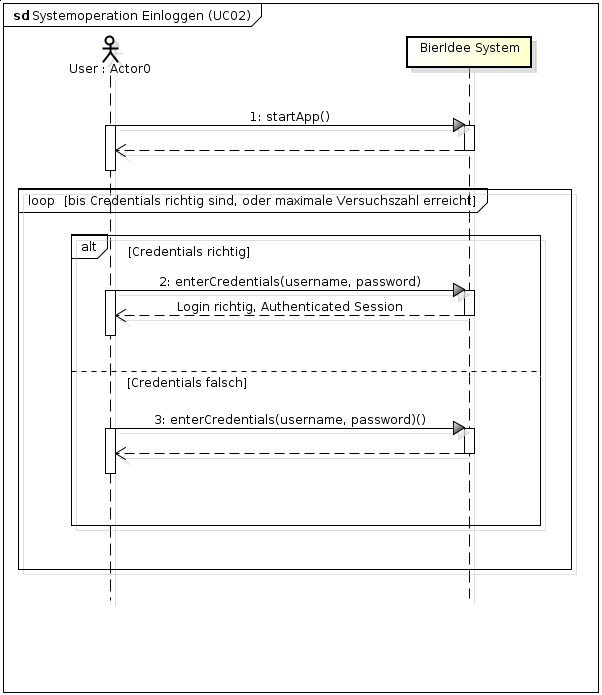
\includegraphics[width=\textwidth]{ssd_uc02.png}

\subsection{Bier bewerten, UC05}
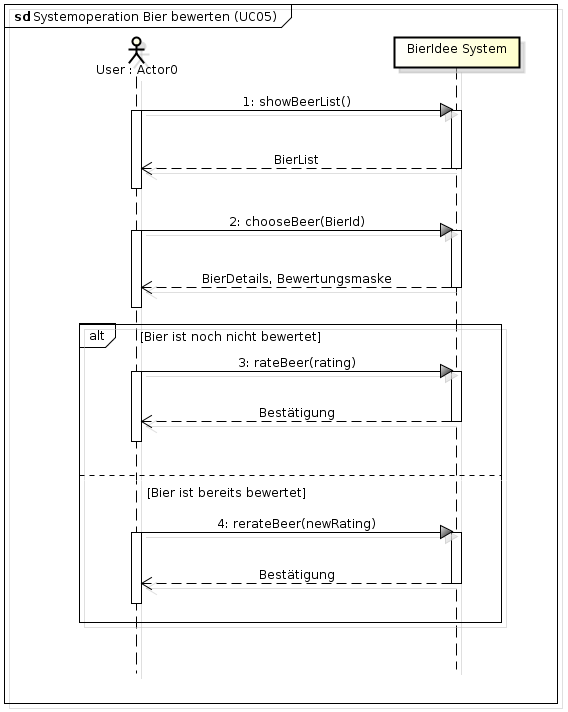
\includegraphics[width=\textwidth]{ssd_uc05.png}

\section{Systemoperationen}
\subsection{Contracts zu Usecase UC02: Einloggen}
\subsubsection{CO01: enterCredentials}
\begin{tabular}{|l|p{0.75\textwidth}|}
\hline
 \textbf{Operation} & enterCredentials(username : String, password: String) \\ 
\hline
\textbf{Cross references} & -- \\ 
\hline 
\textbf{Preconditions} & \begin{itemize} 
							\item Benutzer ist registriert
							\item Benuzerkonto ist aktiviert 
						  \end{itemize}\\
\hline 
\textbf{Postconditions} & Authentiserte Session wurde erstellt \\
\hline
\end{tabular}


\subsection{Contracts zu Usecase UC05: Bier bewerten}
\subsubsection{CO02: showBeerList}
\begin{tabular}{|l|p{0.75\textwidth}|}
\hline
 \textbf{Operation} & showBeerList() \\ 
\hline
\textbf{Cross references} & \begin{itemize}
								\item Bier bearbeiten (UC04)
								\item Bier taggen (UC06)
								\item Bierkatalog abrufen (UC08)
								\item Konsum erfassen (UC10)
							\end{itemize} \\ 
\hline 
\textbf{Preconditions} & \begin{itemize}
							\item Benuzer ist angemeldet
							\item Biere sind erfasst 
						 \end{itemize}\\
\hline 
\textbf{Postconditions} & -- \\
\hline
\end{tabular}

\subsubsection{CO03: chooseBeer}
\begin{tabular}{|l|p{0.75\textwidth}|}
\hline
 \textbf{Operation} & chooseBeer(beer : Beer) \\ 
\hline
\textbf{Cross references} & \begin{itemize}
								\item Bier bearbeiten (UC04)
								\item Bier taggen (UC06)
								\item Konsum erfassen (UC10)
						    \end{itemize} \\ 
\hline 
\textbf{Preconditions} & \begin{itemize}
							\item Benuzer ist angemeldet
							\item Biere sind erfasst 
						 \end{itemize} \\
\hline 
\textbf{Postconditions} & -- \\
\hline
\end{tabular}

\subsubsection{CO04: rateBeer}
\begin{tabular}{|l|p{0.75\textwidth}|}
\hline
 \textbf{Operation} & rateBeer(ratingValue : Integer) \\ 
\hline
\textbf{Cross references} & -- \\ 
\hline 
\textbf{Preconditions} & \begin{itemize}
							\item Benuzer ist angemeldet
							\item Biere sind erfasst 
						 \end{itemize}\\
\hline 
\textbf{Postconditions} & \begin{itemize}
							\item Neue Bewertung wird erstellt
							\item Neue Aktivität wird dem Benuzer zugeordnet
							\item Neue Aktivität wird dem Bier zugeordnet
						  \end{itemize} \\
\hline
\end{tabular}


\end{document}